\section{Vectores aleatorios}

\subsection{Introducción}

\lb{Objetivo: }estudiar $k$ variables sobre una población de individuos (objetos).

\lb{Algunos ejemplos:}
\begin{itemize}[label=$\to$]
\item Las variables meteorológicas como temperatura, humedad y velocidad del viento.
\item La intensidad y la fase de una señal aleatoria que se miden en los canales de comunicación.
\item Los parámetros clínicos de los pacientes (como presión arterial, niveles de glucosa, etc.)
\end{itemize}
Habitualmente estas variables cualitativas o discretas que nos indicarán grupos de individuos.

Estas variables se representarán mediante vectores aleatorios sobre un espacio de probabilidad.

\begin{enumerate}[label=\arabic*)]
	\item Definiciones
\end{enumerate}

Un \lb{vector aleatorio} (v.a.) $k$-dimensional sobre un espacio de probabilidad $(\Omega,\mathcal{S},\mathcal{P})$ es $X=(X_1,\dots,X_k)$ tal que \[ X_i^{-1}(-\infty,x]\in\mathcal{S} \]para todo $x\in\R,\, i=1,\dots,k$

\begin{itemize}[label=\color{red}\textbullet, leftmargin=*]
	\item \color{lightblue}Función de distribución conjunta
\end{itemize}

$F:\R^k\longrightarrow[0,1],$\[ F(x_1,\dots,x_k)\coloneq P[X_1\le x_1,X_2\le x_2,\dots,X_k\le x_k], \] para todo $x_1,\dots,x_k\in\R$.

\subsection{Independencia de las variables aleatorias}

\begin{itemize}[label=\color{red}\textbullet, leftmargin=*]
	\item \color{lightblue}Definición
\end{itemize}
Las variables aleatorias $X_1,\dots,X_k$ son \lb{independientes} si los sucesos \[ \{x_1\le x_1\},\{X_2\le x_2\},\dots,\{X_k\le x_k\} \]son independientes para todo $x_1,\dots,x_k\in\R$.

Esto es equivalente a que \[ F(x_1,\dots,x_k)=P[X_1\le x_1]\cdot P[X_2\le x_2]\cdots P[X_k\le x_k] \]para todo $x_1,\dots,x_k\in\R$.


\subsection{Distribuciones marginales}

La función $F_{X_i}(x_i)=P[X_i\le x_i]$ se denomina \lb{función de distribución marginal} $i$-ésima y corresponde con la función de distribución de la variable aleatoria $X_i$

Las \lb{distribuciones marginales} pueden obtenerse a partir de la distribución conjunta: \[ F_{X_i}(x_I)=F(+\infty,\dots,+\infty,x_i,+\infty,\dots,+\infty) \]
Análogamente, la \lb{función de distribución marginal del subvector aleatorio} $(X_{i_1},\dots,X_{i_m})$ vendrá dada por \[ F_{X_{i_1},\dots,X_{i_m}}(x_{i_1},\dots,x_{i_m})=F(+\infty,\dots,+\infty,x_{i_1},+\infty,\dots,+\infty,x_{i_m},+\infty,\dots,+\infty). \]

\subsection{Vector aleatorio absolutamente continuo}

Un \vea $X$ es \lb{absolutamente continuo} si existe una función $f:\R^k\longrightarrow\R$ no negativa (llamada \lb{función de densidad}) tal que \[ F(x)=F(x_1,\dots,x_k)=\int_{-\infty}^{x_1}\cdots\int_{-\infty}^{x_k}f(z_1,\dots,z_k)\mathrm{d}z_k,\dots,\mathrm{d}z_1, \]para todo $x=(x_1,\dots,x_k)\in\R^k$

Usando el \lb{teorema fundamental del cálculo}, se tiene que en cada punto de continuidad $(x_1,\dots,x_k)$ de $f$: \[ \dfrac{\partial^kF(x_1,\dots,x_k)}{\partial x_1,\dots,\partial x_k}=f(x_1,\dots,x_k).\]

\begin{tikzpicture}
	\node[red, draw=red, fill=red!10, line width=1.5, text width=\textwidth] {Existen \vas cuya función de distribución es continua pero que no son absolutamente continuas (tienen una parte singular) y puede ocurrir que $X_1,\dots,X_k$ sean absolutamente continuas y que $(X_1,\dots,X_k)$ no lo sea.
	\begin{itemize}[label=$\to$]
	\item Ejemplo: Si $X_1$ es una \va absolutamente continua, entonces el \vea $X=(X_1,X_2)$ es continuo pero no absolutamente continuo.
	
	\item De hecho, es completamente singular ya que está contenido en la recta $y=x$ que tiene medida cero en $\R^2$.
	\end{itemize}
	Esto ocurre si consideramos las notas de unos alumnos y sus medidas. En estos casos deberemos eliminar estas variables dependientes del vector.
	};
\end{tikzpicture}

\subsection{Vector aleatorio discreto}
Un vector aleatorio $X$ se dice que es \lb{discreto} si existe un conjunto numerable $\mathcal{S}\in\R^k$ tal que $P(X\in\mathcal{S})=1$.

\lb{Función masa de probabilidad} de una vector aleatorio discreto: \[ P[X=x]=P[X_1=x_1,\dots,X_k=x_k] \]para todo $x=(x_1,\dots,x_k)\in\R^k$, satisfaciendo:
\begin{itemize}[label=$\to$]
\item $P[X=x]\ge0,\;\forall x\in\mathcal{S}$
\item $\sum_{x\in\mathcal{S}}P[X=x]=1$
\end{itemize}
\lb{Función de distribución} de un \vea discreto: \[ F(x)=P[X\le x]=\sum_{\begin{subarray}{c}
z\in\mathcal{S}\\
z\le x
\end{subarray}}P[X=z], \]para todo $x\in\R^k$.

\subsection{Distribuciones marginales}
\subsubsection{Caso continuo}
\begin{itemize}[label=\color{red}\textbullet, leftmargin=*]
	\item \color{lightblue}Distribución marginal de la variable aleatoria $X_i$
\end{itemize}
Sea $X=(X_1,\dots,X_k)$ un \vea continuo con función de densidad $f$ entonces cada componente $X_i$ es de tipo continuo y su función de distribución es; \[ F_{X_i}(x_i)=P[X_i\le x_i]=\int_{-\infty}^{x_i}f_{X_i}(z_i)\mathrm{d}z_i, \]con\[ f_{X_i}=\int_{-\infty}^{+\infty}\cdots\int_{-\infty}^{+\infty}f(z_1,\dots,z_k)\mathrm{d}z_1,\dots,\mathrm{d}z_{i-1}\cdot\mathrm{d}z_{i+1}\dots,\mathrm{d}z_k, \]para todo $z_i\in\R$.

La función de densidad marginal de cualquier subvector se calcularía de igual forma.

$X_1,\dots,X_k$ son \lb{independientes} $\longleftrightarrow f(x_1,\dots,x_k)=f_{X_1}(x_1)\cdots f_{X_k}(x_k)$.

\subsubsection{Caso discreto}
\begin{itemize}[label=\color{red}\textbullet, leftmargin=*]
	\item \color{lightblue}Distribución marginal de la variable aleatoria $X_i$
\end{itemize}
Sea $X=(X_1,\dots,X_l)$ un vector aleatorio discreto con $P[X\in\mathcal{S}]=1$ y función masa de probabilidad $P[X=x]$, para todo $x\in\mathcal{S}$.

Si $X_i$ es una componente arbitraria y por tanto discreta con valores en $\mathcal{S}_i$, entonces su \lb{función masa de probabilidad} puede obtenerse a partir de la conjunta: \[ P[X_i=x_i]=\sum_{\begin{subarray}{c}
x_1\dots,x_{i-1},x_{i+1},\dots,x_k\\
(x_1,\dots,x_i,\dots,x_n)\in\mathcal{S}
\end{subarray}}P[X_1=x_1,\dots,X_{i-1}=x_{i-1},X_i=x_i,X_{i+1}=x_{i+1},\dots,X_k=x_k]. \]

La función masa de probabilidad marginal de cualquier subvector se calcularía de igual forma.

$X_1,\dots,X_k$ son \lb{independientes} $\longleftrightarrow$ para todo $(x_1,\dots,x_k)\in\mathcal{S},$ \[ P[X_1=x_1,\dots,X_k=x_k]=P[X_1=x_1]\cdots P[X_k=x_k]. \]

\begin{tikzpicture}
	\node[red, draw=red, fill=red!10, line width=1.5, text width=10cm] {\underline{Nota:}\\
	$A$ y $B$ independientes $\longleftrightarrow P(A|B)=P(A)$\\
	$P(A|B)=\dfrac{P(A\cap B)}{P(B)}=P(A)\longrightarrow P(A\cap B)=P(A)\cdot P(B)$
	};
\end{tikzpicture}
\subsection{Distribuciones condicionadas}
\subsubsection{Caso continuo}

\begin{itemize}[label=\color{red}\textbullet, leftmargin=*]
	\item \color{lightblue}Distribución condicionada al valor de una variable
\end{itemize}

Sea $X=(X_1,\dots,X_k)$ un vector aleatorio continuo con función de densidad $f$.\\
Sea $X_i$ una componente arbitraria y $x_i^*\in\R$ tal que $f_{X_i}(x_i^*)>0$.\\
Se define la \lb{distribución condicionada} de $(X_1,\dots,X_{i-1},X_{i+1},\dots,X_k)$ a $(X_i=x_i^*)$ como la determinada por la función de densidad:

\[ f_{X_1,\dots,X_{i-1},\dots,X_k|X_i=x_i^*}(x_1,\dots,x_{i-1},x_{i+1},\dots,x_k|x_i^*)=\dfrac{f(x_1,\dots,x^*,\dots,x_k)}{f_{X_i}(x_i^*)}. \]


\begin{itemize}[label=\color{red}\textbullet, leftmargin=*]
	\item \color{lightblue}Distribución condicionada a valores de varias variables
\end{itemize}
Sea $X=(X_1,\dots,X_k)$ un vector aleatorio continuo con función de densidad $f$.\\
Sea $(X_{i_1},\dots,X_{i_m})$ un subvector arbitrario y $(x_{i_1}^{*},\dots,x_{i_m}^*)\in\R^m$ tal que: \[ f_{X_{i_1},\dots,X_{i_m}}(x_{i_1}^*,\dots,x_{i_m}^*)>0. \]
Se define la \lb{distribución condicionada} de $(X_1,\dots,X_{i_{1}-1},X_{i_1+1},\dots,X_{i_m-1};X_{i_m+1},\dots,X_k)$ a $(X_{i_1}=x_{i_1}^*,\dots,X_{i_m}=x_{i_m^*})$ como la determinada por la función de densidad:
\[ f_{X_1,\dots,X_{i_{1}-1},X_{i_1+1},\dots,X_{i_m-1},\dots,X_k|X_{i_1}=x_{i_1}^*,\dots,X_{i_m}=x_{i_m^*}}(x_1,\dots,x_{i-1},x_{i+1},\dots,x_{i_m-1},x_{i_m+1},\dots,x_k|x_i^*)=\dfrac{f(x_1,\dots,x_{i_1}^*,\dots,x_{i_m}^*\dots,x_k)}{f_{X_{i_1},\dots,X_{i_m}}(x_{i_1}^*,\dots,x_{i_m}^*)} \]
\subsubsection{Caso discreto}
\begin{itemize}[label=\color{red}\textbullet, leftmargin=*]
	\item \color{lightblue}Distribución condicionada al valor de una variable
\end{itemize}
Sea $X=(X_1,\dots,X_k)$ un vector aleatorio discreto.\\
Sea $X_i$ una componente arbitraria y $x_i^*\in\R$ tal que \[ P[X_i=x_i^*]>0. \]
Se define la \lb{distribución condicionada} de $(X_1,\dots,X_{i-1},X_{i+1},\dots,X_k)$ a $(X_i=x_i^*)$ como la determinada por la función masa de probabilidad:

\begin{center}
$P[X_1=x_1,\dots,X_{i-1}=x_{i-1},X_{i+1}=x_{i+1},\dots,X_k=x_k|X_i=x_i^*]=\dfrac{P[X_1=x_1,\dots,X_{i-1}=x_{i-1},X_i=x_i^*,X_{i+1}=x_{i+1},\dots,X_k=x_k]}{P[X_i=x_i^*]} $
\end{center}

para todo $(x_1,\dots,x_{i-1},x_{i+1},\dots,x_k)$ tal que $x_1,\dots,x_{i-1},x_i^*,x_{i+1},\dots,x_k\in\mathcal{S}$.

\begin{itemize}[label=\color{red}\textbullet, leftmargin=*]
	\item \color{lightblue}Distribución condicionada a valores de varias variables
\end{itemize}
Sea $X=(X_1,\dots,X_k)$ un vector aleatorio discreto.

Sea $X_{i_1},\dots,X_{i_m}$ un subvector arbitrario y $(x_{i_1}^*,\dots,x_{i_m}^*)\in\R^m$ tal que \[ P[X_{i_1}=x_{i_1}^*,\dots,X_{i_m}=x_{i_m}^*]>0. \]
Se define la \lb{distribución condicionada} de $(X_1,\dots,X_{i_1-1},X_{i_1+1},\dots,X_{i_m-1},X_{i_m+1},\dots,X_k)$ a $(X_{i_1}=x_{i_1}^*,\dots,X_{i_m}=x_{i_m}^*)$ como la determinada por la función masa de probabilidad:

\begin{center}
$P[X_1=x_1,\dots,X_{i_{1}-1}=x_{i_1-1},X_{i_1+1}=x_{i_1+1},\dots,X_{i_m-1}=x_{i_m-1},X_{i_m+1}=x_{i_m+1},\dots,X_k=x_k|X_{i_1}=x_{i_1}^*,\dots,X_{i_m}=x_{i_m^*}]=\dfrac{P[X_1=x_1,\dots,X_{i_1}=x_{i_1}^*,\dots,X_{i_m}=x_{i_m}^*,\dots,X_k=x_k]}{P[X_{i_1}=x_{i_1}^*,\dots,X_{i_m}=x_{i_m}^*]}$
\end{center}
para todo $(x_1,\dots,x_{i_1},x_{i_1+1},\dots,x_{i_m-1},x_{i_m+1},\dots,x_k)$, tal que $(x_1,\dots,x_{i_1}^*,\dots,x_{i_m}^*,\dots,x_k)\in\mathcal{S}$

\subsection{Distribución normal multivariante $\mathcal{N}_k(\mu,V)$}
\begin{enumerate}[label=\arabic*)]
	\item Función de densidad
\end{enumerate}
\[ f(x)=\dfrac{1}{\sqrt{|V|(2\pi)^k}}\exp\left(-\dfrac{1}{2}(x-\mu)'V^{-1}(x-\mu)\right), \]para $x\in\R^k$, donde $\mu$ es un vector $k$-dimensional y $V$ es una matriz $k\times k$ simétrica y definida positiva.

\begin{itemize}[label=\color{red}\textbullet, leftmargin=*]
	\item \color{lightblue}Definiciones
\end{itemize}
Una matriz simétrica $A$, de dimensión $k\times k$, se dice que es \lb{definida positiva} si se verifica que $x'Ax>0$ para cualquier vector no nulo $x\in\R^k$.

Una matriz simétrica $A$, de dimensión $k\times k$, se dice que es \lb{semidefinida positiva} si se verifica que $x'Ax\ge0$ para cualquier vector $x\in\R^k$.

¿Cómo calcular la inversa de $V=\begin{pmatrix}
1 & \tfrac{1}{2}\\
\tfrac{1}{2} & 1
\end{pmatrix}$ con \lb{\texttt{R}}?

\vspace{0.5cm}

\begin{lstlisting}
V <- matrix(c(1, 1/2,
						1/2, 1), nrow = 2, ncol = 2, byrow = TRUE)
solve(V)
\end{lstlisting}

\begin{verbatim}
##            [,1]       [,2]
## [1,]  1.3333333 -0.6666667
## [2,] -0.6666667  1.3333333
\end{verbatim}

\subsubsection{Normal bivariante}
\begin{itemize}[label=\color{red}\textbullet, leftmargin=*]
	\item \color{lightblue}Función de densidad
\end{itemize}
Caso bivariante, $k=2$, para $\mu=(0,0)$ y $V=\begin{pmatrix}
1 & \tfrac{1}{2}\\
\tfrac{1}{2} & 1
\end{pmatrix}$.

Cálculo de la función de densidad en $x=(1,1)$ utilizando la función \lb{\texttt{dmvnorm}} de la librería \lb{\texttt{mvtnorm}} de \lb{\texttt{R}}:

\begin{lstlisting}
library("mvtnorm")
V <- matrix(c(1, 1/2,
              1/2, 1), nrow = 2, ncol = 2, byrow = TRUE)
mu <- c(0, 0)
x <- c(1, 1)
dmvnorm(x, mean = mu, sigma = V)
\end{lstlisting}

\begin{verbatim}
## [1] 0.0943539
\end{verbatim}
\begin{itemize}[label=\color{red}\textbullet, leftmargin=*]
	\item \color{lightblue}Función de distribución
\end{itemize}
Cálculo (aproximado) de la función de distribución en $x=(1,1)$ con la función: 

\lb{\texttt{pmvnorm(lower = -Inf, upper = x, mean = mu, sigma = V)}}

\begin{lstlisting}
library("mvtnorm")
V <- matrix(c(1, 1/2,
              1/2, 1), nrow = 2, ncol = 2, byrow = TRUE)
mu <- c(0, 0)
x <- c(1, 1)
pmvnorm(lower = -Inf, upper = x, mean = mu, sigma = V)
\end{lstlisting}

\begin{verbatim}
## [1] 0.7452036
\end{verbatim}

\begin{itemize}[label=\color{red}\textbullet, leftmargin=*]
	\item \color{lightblue}Probabilidad en rectángulos
\end{itemize}
Cálculo (aproximado) de las probabilidades en rectángulos dando los límites inferiores y superiores del rectángulo. Por ejemplo, para calcular \[ P(-1<X_1<1,\:-1<X_2<1) \]
\begin{lstlisting}
library("mvtnorm")
V <- matrix(c(1, 1/2,
              1/2, 1), nrow = 2, ncol = 2, byrow = TRUE)
mu <- c(0, 0)
x1 <- c(- 1, -1)
x2 <- c(1, 1)
pmvnorm(lower = x1, upper = x2, mean = mu, sigma = V)
\end{lstlisting}

\begin{verbatim}
## [1] 0.499718
\end{verbatim}

Su representación gráfica:

\begin{lstlisting}
f <- function(x1, x2) dmvnorm(data.frame(x1, x2), mu, V)
x <- seq(-3, 3, length = 50)
y <- seq(-3, 3, length = 50)
z <- outer(x, y, f)
persp(x, y, z, xlab = 'x1', ylab = 'x2', zlab = 'f(x1, x2)', col = 'orange', main = "Función de densidad")
\end{lstlisting}

\begin{center}
\includegraphics{"Temas/Imágenes/Tema 1/000012.png"}
\end{center}

Su representación gráfica $\left(f(x_1,x_2)=c\right)$ y 50 datos simulados de este modelo

\begin{lstlisting}
#Se fija la semilla para la generación aleatoria
set.seed(123)
#Generación aleatoria del modelo
d <- rmvnorm(50, mu, V)
plot(d, xlab = "X1", ylab = "X2", pch = 20, xlim = c(-3, 3), ylim = c(-3, 3))
contour(x, y, z, nlevels = 4, add = T, col = 'red')
\end{lstlisting}

\begin{center}
\includegraphics{"Temas/Imágenes/Tema 1/000014.png"}
\end{center}

\begin{itemize}[label=\color{red}\textbullet, leftmargin=*]
	\item \color{lightblue}Distancia de Mahalanobis
\end{itemize}

La distancia de Mahalanobis del vector $x$ al vector $\mu$ basada en la matriz $V$: \[ D=\sqrt{(x-\mu)'V^{-1}(x-\mu)} \]
Tiene en cuenta la diferentes escalas de los datos y sus correlaciones.

Servirá para detectar las observaciones más alejadas del vector de medias que podrían ser observaciones atípicas (\lb{\texttt{outliers}}) que no provengan de nuestra población o contengan errores.
\begin{itemize}[label=$\to$]
\item Cuando se pueda, se deberán chequear y, si es posible, corregir o eliminar.
\item En otros casos, se deberán mantener por ser observaciones correctas que hay que tener en cuenta.
\end{itemize}
\begin{itemize}[label=\color{red}\textbullet, leftmargin=*]
	\item \color{lightblue}Cálculo de la distancia de Mahalanobis
\end{itemize}


Para calcular las distancias de Mahalanobis al cuadrado de los datos al vector de medias (teóricas o muestrales) podemos utilizar la función \lb{\texttt{mahalanobis}}.

\begin{lstlisting}
V <- matrix(c(1, 1/2,
              1/2, 1), nrow = 2, ncol = 2, byrow = TRUE)
mu <- c(0, 0)
dM1 <- mahalanobis(d, mu, V)
dM2 <- mahalanobis(d, colMeans(d), cov(d))
\end{lstlisting}

\begin{itemize}[label=\color{red}\textbullet, leftmargin=*]
	\item \color{lightblue}Distancias de los datos simulados al vector de medias teóricas $\mu$ con respecto a $V$
\end{itemize}

\begin{lstlisting}
summary(dM1)
\end{lstlisting}

\begin{verbatim}
##    Min. 1st Qu.  Median    Mean 3rd Qu.    Max. 
## 0.05216 0.41016 1.26433 1.66615 2.31591 7.13332
\end{verbatim}

\begin{itemize}[label=\color{red}\textbullet, leftmargin=*]
	\item \color{lightblue}¿Dónde se encuentra la observación más alejada del vector de medias?
\end{itemize}

\begin{lstlisting}
d[which.max(dM1), ]
\end{lstlisting}

\begin{verbatim}
## [1] 2.509470 2.046512
\end{verbatim}

\begin{lstlisting}
f <- function(x1, x2) dmvnorm(data.frame(x1, x2), mu, V)
x <- seq(-3, 3, length = 50)
y <- seq(-3, 3, length = 50)
z <- outer(x, y, f)
plot(d, xlab = "X1", ylab = "X2", pch = 20, xlim = c(-3, 3), ylim = c(-3, 3))
points(d[which.max(dM1), 1], d[which.max(dM1), 2], col = "blue", pch = 8)
text(d[which.max(dM1), 1], d[which.max(dM1), 2], which.max(dM1), cex = 0.8, pos = 3)
contour(x, y, z, nlevels = 4, add = T, col = 'red')
\end{lstlisting}

\begin{center}
\includegraphics{"Temas/Imágenes/Tema 1/000014.png"}
\end{center}
\begin{itemize}[label=\color{red}\textbullet, leftmargin=*]
	\item \color{lightblue}Distancias de los datos simulados al vector de medias muestrales $\overline{x}$ con respecto a $\mathcal{S}$
\end{itemize}
\begin{lstlisting}
summary(dM2)
\end{lstlisting}

\begin{verbatim}
##    Min. 1st Qu.  Median    Mean 3rd Qu.    Max. 
## 0.02114 0.67111 1.52636 1.96000 2.64131 8.65906
\end{verbatim}

\begin{itemize}[label=\color{red}\textbullet, leftmargin=*]
	\item \color{lightblue}¿Dónde se encuentra la observación más alejada del vector de medias?
\end{itemize}

\begin{lstlisting}
d[which.max(dM2), ]
\end{lstlisting}

\begin{verbatim}
## [1] 2.509470 2.046512
\end{verbatim}

\begin{lstlisting}
f <- function(x1, x2) dmvnorm(data.frame(x1, x2), colMeans(d), cov(d))
x <- seq(-3, 3, length = 50)
y <- seq(-3, 3, length = 50)
z <- outer(x, y, f)
plot(d, xlab = "X1", ylab = "X2", pch = 20, xlim = c(-3, 3), ylim = c(-3, 3))
points(d[which.max(dM2), 1], d[which.max(dM2), 2], col = "blue", pch = 8)
text(d[which.max(dM2), 1], d[which.max(dM2), 2], which.max(dM2), cex = 0.8, pos = 3)
contour(x, y, z, nlevels = 4, add = T, col = 'magenta')
\end{lstlisting}

\begin{center}
\includegraphics{"Temas/Imágenes/Tema 1/000015.png"}
\end{center}
\subsection{Distribución multinomial $\mathcal{M}_k(n,p_1,\dots,p_k)$}
\begin{itemize}[label=\color{red}\textbullet, leftmargin=*]
	\item \color{lightblue}Modelo multinomial
\end{itemize}
$(X_1,\dots,X_k)$: variables aleatorias que representan el número de veces que ocurre el suceso $A_i$ en un experimento aleatorio repetido $n$ veces con $k$ opciones dadas por $\{A_1,\dots,A_k\}$ y con probabilidades constantes $p_i=P(A_i)$, para $i=1,\dots,k$.
\lb{Función masa de probabilidad conjunta:} \[ p(x_1,\dots,x_k)=P[X_1=x_1,\dots,X_k=x_k]=\dfrac{n!}{x_1!\cdots x_k!}p_1^{x_1}\cdots p_k^{x_k}, \] para enteros no negativos tales que $x_1+\cdots+x_k=n$ y donde $p_i\in[0,1]$ satisface $p_1+\cdots+p_k=1$.

\lb{Distribuciones marginales:} $X_i$ sigue una distribución binomial $B(n,p_i)$, con $E(X_i)=np_i$.
\subsection{Estadístico de Pearson}
\begin{itemize}[label=\color{red}\textbullet, leftmargin=*]
	\item \color{lightblue}Discrepancias entre lo observado y lo esperado
\end{itemize}
\lb{Contexto:} Lanzamos un dado $n=$ veces, $p_i=\frac{1}{6}$ para todo $i$, y los valores esperados son $np_i=10$, para $i=1,\dots,6$.

\lb{Objetivo:} Medir las discrepancias entre valores observados y esperados.

Sea $X=(X_1,\dots,X_k)$ una \va con distribución multinomial, entonces el estadístico \[ T=\sum_{i=1}^{k}\dfrac{X_i-np_i}{np_i} \]sigue una distribución Chi-cuadrado $\chi_{k-1}^2$ de Pearson con $k-1$ grados de libertad, cuando $n\longrightarrow\infty$.
\subsection{Medias y covarianzas}
\begin{itemize}[label=\color{red}\textbullet, leftmargin=*]
	\item \color{lightblue}Definiciones
\end{itemize}
Dado el vector aleatorio.
\begin{itemize}[label=$\to$]
\item El \lb{vector de medias} (o \lb{esperanza matemática} de $X$) se define como: \[ \mu\coloneq E[X]=(E[X_1],\dots,E[X_k])'=(\mu_1,\dots,\mu_k)' \](note que es un vector columna).
\item La \lb{matriz de covarianzas (o varianzas-covarianzas)} se define como: \[ V=(\sigma_{i,j}), \] donde $\sigma_{i,j}$ es la covarianza entre $X_i$ y $X_j$, definida como: \[ \sigma_{i,j}=\cov(X_i,X_j)=E\left[(X_i-\mu_i)(X_j-\mu_j)\right]=E[X_iX_j]-\mu_i\mu_j \]Notemos que $\sigma_{i,i}=E\left[(X_i-\mu_i)^2\right]=\var(X_i)=\sigma_i^2$.
\end{itemize}
\begin{itemize}[label=\color{red}\textbullet, leftmargin=*]
	\item \color{lightblue}Cálculo de la esperanza matemática
\end{itemize}
La media de cada componente $X_i$ del vector puede calcularse a partir de la distribución conjunta o a partir de la marginal.
\begin{itemize}[label=\color{lightblue}$\to$]
\item \lb{Caso discreto:} \[ \begin{aligned}
E[X_i]&=\sum_{x_i}x_i P[X_i=x_i]\\
&=\sum_{x_1,\dots,x_k}x_i P[X_1=x_1,\dots,X_k=x_k]
\end{aligned} \]
\item \lb{Caso continuo:} \[ \begin{aligned}
E[X_i] &=\int_{\R }x_if_{X_i}(x_i)\dx_i\\
&=\int_{\R^k}x_if(x_1,\dots,x_k)\dx_1\cdots\dx_k
\end{aligned} \]
\end{itemize}

\subsubsection{Esperanza de la transformación $g:\R^k\longrightarrow\R$}
\begin{itemize}[label=\color{red}\textbullet, leftmargin=*]
	\item \color{lightblue}Caso discreto
\end{itemize}
Sea $g:\R^k\longrightarrow\R$ una función medible $\longrightarrow Y=g(X)$ es una \va. 

Si $X$ es de tipo discreto, \[ \exists E[g(X)]\longleftrightarrow\sum_{x_1,\dots,x_k}\left|g(x_1,\dots,x_k)\right|P[X_1=x_1,\dots,X_k=x_k]<\infty \]
Y en caso de existir: \[ E[g(X_1,\dots,X_k)]=\sum_{x_1,\dots,x_k}g(x_1,\dots,x_k)P[X_1=x_1,\dots,X_k=x_k] \]
\begin{itemize}[label=\color{red}\textbullet, leftmargin=*]
	\item \color{lightblue}Caso continuo
\end{itemize}
Sea $g:\R^k\longrightarrow\R$ una función medible $\longrightarrow Y=g(X)$ es una \va.

Si $X$ es de tipo continuo, \[ \exists E[g(X)]\longleftrightarrow\int_{\R^k}\left|g(x_1,\dots,x_k)\right|f_X(x_1,\dots,x_k)\dx_1\cdots\dx_k<\infty \]
Y en caso de existir: \[ E[g(X_1,\dots,X_k)]=\int_{\R^k}g(x_1,\dots,x_k)f_X(x_1,\dots,x_k)\dx_1\cdots\dx_k. \]
\begin{itemize}[label=\color{red}\textbullet, leftmargin=*]
	\item \color{lightblue}Propiedades
\end{itemize}
$V$ es una matriz \lb{simétrica} y \lb{semidefinida positiva} ($x'Vx\ge0$, para todo $x\in\R^k$).

En forma matricial, \[ V=E\left[(X-\mu)(X-\mu)'\right]=E[XX']-\mu\mu'.\] donde la \lb{esperanza de una matriz aleatoria} se define como la matriz de las esperanzas de cada variable.

Si $X_i$ y $X_j$ son \lb{independientes}, entonces \[ E[X_iX_j]=E[X_i]E[X_j] \]y, por lo tanto, $\cov(X_i,X_j)=0$. El recíproco no es cierto.

Si $X\longrightarrow\mathcal{N}_k(\mu, V)$, se puede demostrar que $\mu$ es el vector de medias y $V$ es la matriz de covarianzas.
\subsection{Correlación}
La \lb{correlación (lineal de Pearson)} entre $X_i$ y $X_j$ se define como \[ \rho_{i,j}=\corr(X_i,X_j)=\dfrac{\sigma_{i,j}}{\sigma_i\sigma_j} \]siendo $\rho_{i,i}=\corr(X_i,X_j)=1$.

Mide el \lb{grado de relación lineal} entre $X_i$ y $X_j$.

Puede demostrarse que \[ -1\le\rho_{i,j}\le1. \]
Se dice que $X_i$ y $X_j$ son \lb{incorreladas} si $\rho_{i,j}=0$.

Si son independientes serán incorreladas, pero el recíproco no es cierto.

La \lb{matriz de correlaciones} es $R=(\rho_{i,j})$.
\subsection{Correlación entre vectores aleatorios}
Análogamente, si $X$ e $Y$ son \veas (de dimensiones cualesquiera), se define su \lb{matriz de covarianzas} como \[ \cov(X,Y)=(\cov(X_i,Y_j)) \] y su \lb{matriz de correlaciones} como \[ \corr(X,Y)=(\corr(X_i,Y_j)). \]Puede demostrarse que \[ \cov(X,Y)=E[(X-E[X])(Y-E[Y])']. \]Evidentemente, $\cov(X)=\cov(X,X)$.
\begin{itemize}[label=\color{red}\textbullet, leftmargin=*]
	\item \color{lightblue}Propiedades
\end{itemize}
Si $X,Y,Z$ son vectores (columna) aleatorios, se verifican las propiedades siguientes:
\begin{enumerate}[label=\color{lightblue}\arabic*)]
	\item $E[a_1g_1(X)+a_2g_2(X)]=a_1E[g_1(X)]+a_2E[X_2]$, donde $a_1,a_2\in\R$ y $g_1$ y $g_2$ son funciones medible de vectores aleatorios.
	\item $X=(Y,Z),E_X[g(Y)]=E_Y[g(Y)]$, donde $g$ es una función medible de un vector aleatorio, $E_X$ denota la esperanza en la distribución conjunta y $E_Y$ en la distribución marginal.
	\item Si $X$ e $Y$ son independientes, entonces \[ E[g_1(X)g_2(Y)]=E[g_1(X)]E[g_2(Y)], \] donde $g_1$ y $g_2$ son funciones medibles cualesquiera de \veas.
	\item $E[AX+b]=AE[X]+b,A\in M_{m,k}b'\in\R^m$.
	\item $\cov(X_i,X_j)=E[X_iX_j]-E[X_i]E[X_j]$.
	\item Si $X_1,\dots,X_k$ son independientes, $\cov(X_i,X_j)=0$.
	\item $\var(X_i+X_j)=\var(X_i)+2\cov(X_i,X_j)+\var(X_j)$.
	\item $\cov(aX_i+b,cX_j+d)=ac\cov(X_i,X_j)$, donde $a,b,c,d\in\R$.
	\item $\cov(X)=E[(X-\mu)(X-\mu)']=E[XX']-\mu\mu'$.
	\item $\var(a'X)=a'\cov(X)a=\sum_{i,j}a_ia_j\sigma_{i,j}$, donde $a\in\R^k$.
	\item $\cov(AX+b)=A\cov(X)A'$, donde $A\in M_{m,k}$ y $b'\in\R^m$.
	\item Si $X_1,\dots,X_k$ son independientes, $\corr(X_i,X_j)=0$.
	\item $\corr(aX_i+b,cX_j+d)=\corr(X_i,X_j)$, donde $a,b,c,d\in\R$.
	\item $-1\le\corr(X_i,X_j)\le1$.
	\item $\corr(X_i,aX_i+b)=\pm1$, donde $a,b\in\R$ (según el signo de $a$).
	\item $\corr(X)=\delta^{-1}\cov(X)\delta^{-1}$, donde $\delta$ es la matriz diagonal formada por las desviaciones típicas $\left(\delta=\mathrm{diag}(\sigma_1,\dots,\sigma_k)\right)$.
	\item $\cov(X,Y)=\left(\cov(X_i,Y_j)\right)=\cov(Y,X)'$.
	\item $\cov(X+Z,Y)=\cov(X,Y)+\cov(Z,Y)$
	\item Si $X$ e $Y$ tienen la misma dimensión, entonces $\cov(X+Y)=\cov(X)+\cov(X,Y)+\cov(Y,X)+\cov(Y)$.
	\item $\cov(AX,BY)=A\cov(X,Y)B'$, donde $A$ y $B$ son matrices (de dimensiones adecuadas).
	\item Si $X$ e $Y$ independientes, entonces $\cov(X,Y)=0$.
\end{enumerate}
\begin{itemize}[label=\color{red}\textbullet, leftmargin=*]
	\item \color{lightblue}Demostración apartado (10)
\end{itemize}
Directamente se tiene que: \[ \var(a'X)=\cov(a'X,a'X)=E[a'(X-\mu)(X-\mu)'a]=a\cov(X)a \]
Como consecuencia, se obtiene que la matriz de covarianzas $\cov(X)$ es semidefinida positiva ya que $\var(a'X)\ge0$.

Lo mismo le ocurre a la matriz de correlaciones $\corr(X)$ ya que es la matriz de covarianzas de las \vas tipificadas $Z_i=\dfrac{X_i-\mu_i}{\sigma_i}$.
\subsection{Resultados básicos de la inferencia}
\begin{itemize}[label=\color{red}\textbullet, leftmargin=*]
	\item \color{lightblue}Contexto
\end{itemize}
En la práctica, todas las medidas, varianzas y covarianzas serán desconocidas por lo que tenemos que estimarlas.\\
Para ello dispondremos de una muestra de individuos (objetos) en los que se han medido todas las variables.\\
Proporcionamos resultados básicos de inferencia para poder aplicar las técnicas multivariantes que desarrollaremos en temas posteriores.\\
Se ilustran estos procedimientos de inferencia con conjuntos de datos de \lb{\texttt{R}}, accesibles con \lb{\texttt{data()}}.
\subsubsection{¿Cómo se representan las muestras aleatorias?}

\begin{wrapfigure}[5]{r}{0.4\textwidth}
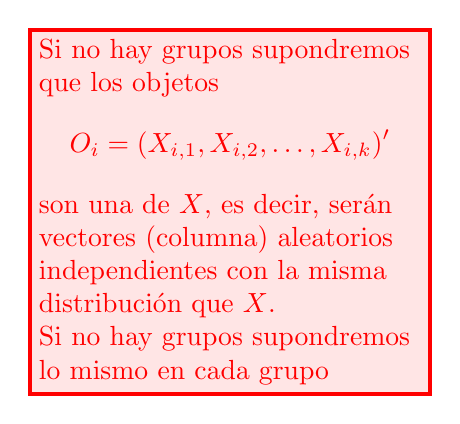
\begin{tikzpicture}
	\node[red, draw=red, fill=red!10, line width=1.5, text width=0.4\textwidth] {Si no hay grupos supondremos que los objetos \[ O_i=(X_{i,1},X_{i,2},\dots,X_{i,k})' \] son una \mas de $X$, es decir, serán vectores (columna) aleatorios independientes con la misma distribución que $X$.\\
	Si no hay grupos supondremos lo mismo en cada grupo
	};
\end{tikzpicture}
\end{wrapfigure}

\begin{itemize}[label=\color{red}\textbullet, leftmargin=*]
	\item \color{lightblue}Matriz de la \mas
\end{itemize}

En general, nuestra muestra aleatoria se representará como:
\[ \begin{array}{cccccc}
i & X_1 & X_2 & \cdots & X_k & Y \\ \hline
O_1 & X_{1,1} & X_{1,2} & \cdots & X_{1,k} & Y_1 \\
\cdots & \cdots & \cdots & \cdots & \cdots & \cdots \\
O_i & X_{i,1} & X_{i,2} & \cdots & X_{i,k} & Y_i \\
\cdots & \cdots & \cdots & \cdots & \cdots & \cdots \\
O_n & X_{n,1} & X_{n,2} & \cdots & X_{n,k} & Y_n \\ \hline
\end{array} \]
La variable $Y$ solo se usará para detonar la variable respuesta en regresión.

En algunos casos usaremos la matriz $M=(X_{i,j})$ que será una matriz aleatoria.
\subsubsection{¿Cómo se muestran los valores muestrales?}

\begin{wrapfigure}[5]{r}{0.4\textwidth}
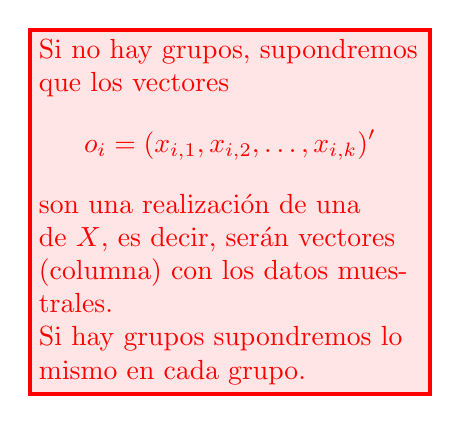
\begin{tikzpicture}
	\node[red, draw=red, fill=red!10, line width=1.5, text width=0.4\textwidth] {Si no hay grupos, supondremos que los vectores \[ o_i=(x_{i,1},x_{i,2},\dots,x_{i,k})' \] son una realización de una \mas de $X$, es decir, serán vectores (columna) con los datos muestrales.\\
	Si hay grupos supondremos lo mismo en cada grupo.
	};
\end{tikzpicture}
\end{wrapfigure}

\begin{itemize}[label=\color{red}\textbullet, leftmargin=*]
	\item \color{lightblue}Matriz de datos
\end{itemize}
En general, nuestra muestra se representará como: 
\[ \begin{array}{cccccc}
i & x_1 & x_2 & \cdots & x_k & y \\ \hline
o_1 & x_{1,1} & x_{1,2} & \cdots & x_{1,k} & y_1 \\
\cdots & \cdots & \cdots & \cdots & \cdots & \cdots \\
o_i & x_{i,1} & x_{i,2} & \cdots & x_{i,k} & y_i \\
\cdots & \cdots & \cdots & \cdots & \cdots & \cdots \\
o_n & x_{n,1} & x_{n,2} & \cdots & x_{n,k} & y_n \\ \hline
\end{array} \]
La variable $Y$ solo se usará para detonar la variable respuesta en regresión.

En algunos casos usaremos la matriz de datos $M=(x_{i,j})$